% Options for packages loaded elsewhere
\PassOptionsToPackage{unicode}{hyperref}
\PassOptionsToPackage{hyphens}{url}
\PassOptionsToPackage{dvipsnames,svgnames,x11names}{xcolor}
%
\documentclass[
  letterpaper,
  DIV=11,
  numbers=noendperiod]{scrreprt}

\usepackage{amsmath,amssymb}
\usepackage{iftex}
\ifPDFTeX
  \usepackage[T1]{fontenc}
  \usepackage[utf8]{inputenc}
  \usepackage{textcomp} % provide euro and other symbols
\else % if luatex or xetex
  \usepackage{unicode-math}
  \defaultfontfeatures{Scale=MatchLowercase}
  \defaultfontfeatures[\rmfamily]{Ligatures=TeX,Scale=1}
\fi
\usepackage{lmodern}
\ifPDFTeX\else  
    % xetex/luatex font selection
\fi
% Use upquote if available, for straight quotes in verbatim environments
\IfFileExists{upquote.sty}{\usepackage{upquote}}{}
\IfFileExists{microtype.sty}{% use microtype if available
  \usepackage[]{microtype}
  \UseMicrotypeSet[protrusion]{basicmath} % disable protrusion for tt fonts
}{}
\makeatletter
\@ifundefined{KOMAClassName}{% if non-KOMA class
  \IfFileExists{parskip.sty}{%
    \usepackage{parskip}
  }{% else
    \setlength{\parindent}{0pt}
    \setlength{\parskip}{6pt plus 2pt minus 1pt}}
}{% if KOMA class
  \KOMAoptions{parskip=half}}
\makeatother
\usepackage{xcolor}
\setlength{\emergencystretch}{3em} % prevent overfull lines
\setcounter{secnumdepth}{5}
% Make \paragraph and \subparagraph free-standing
\makeatletter
\ifx\paragraph\undefined\else
  \let\oldparagraph\paragraph
  \renewcommand{\paragraph}{
    \@ifstar
      \xxxParagraphStar
      \xxxParagraphNoStar
  }
  \newcommand{\xxxParagraphStar}[1]{\oldparagraph*{#1}\mbox{}}
  \newcommand{\xxxParagraphNoStar}[1]{\oldparagraph{#1}\mbox{}}
\fi
\ifx\subparagraph\undefined\else
  \let\oldsubparagraph\subparagraph
  \renewcommand{\subparagraph}{
    \@ifstar
      \xxxSubParagraphStar
      \xxxSubParagraphNoStar
  }
  \newcommand{\xxxSubParagraphStar}[1]{\oldsubparagraph*{#1}\mbox{}}
  \newcommand{\xxxSubParagraphNoStar}[1]{\oldsubparagraph{#1}\mbox{}}
\fi
\makeatother


\providecommand{\tightlist}{%
  \setlength{\itemsep}{0pt}\setlength{\parskip}{0pt}}\usepackage{longtable,booktabs,array}
\usepackage{calc} % for calculating minipage widths
% Correct order of tables after \paragraph or \subparagraph
\usepackage{etoolbox}
\makeatletter
\patchcmd\longtable{\par}{\if@noskipsec\mbox{}\fi\par}{}{}
\makeatother
% Allow footnotes in longtable head/foot
\IfFileExists{footnotehyper.sty}{\usepackage{footnotehyper}}{\usepackage{footnote}}
\makesavenoteenv{longtable}
\usepackage{graphicx}
\makeatletter
\newsavebox\pandoc@box
\newcommand*\pandocbounded[1]{% scales image to fit in text height/width
  \sbox\pandoc@box{#1}%
  \Gscale@div\@tempa{\textheight}{\dimexpr\ht\pandoc@box+\dp\pandoc@box\relax}%
  \Gscale@div\@tempb{\linewidth}{\wd\pandoc@box}%
  \ifdim\@tempb\p@<\@tempa\p@\let\@tempa\@tempb\fi% select the smaller of both
  \ifdim\@tempa\p@<\p@\scalebox{\@tempa}{\usebox\pandoc@box}%
  \else\usebox{\pandoc@box}%
  \fi%
}
% Set default figure placement to htbp
\def\fps@figure{htbp}
\makeatother
% definitions for citeproc citations
\NewDocumentCommand\citeproctext{}{}
\NewDocumentCommand\citeproc{mm}{%
  \begingroup\def\citeproctext{#2}\cite{#1}\endgroup}
\makeatletter
 % allow citations to break across lines
 \let\@cite@ofmt\@firstofone
 % avoid brackets around text for \cite:
 \def\@biblabel#1{}
 \def\@cite#1#2{{#1\if@tempswa , #2\fi}}
\makeatother
\newlength{\cslhangindent}
\setlength{\cslhangindent}{1.5em}
\newlength{\csllabelwidth}
\setlength{\csllabelwidth}{3em}
\newenvironment{CSLReferences}[2] % #1 hanging-indent, #2 entry-spacing
 {\begin{list}{}{%
  \setlength{\itemindent}{0pt}
  \setlength{\leftmargin}{0pt}
  \setlength{\parsep}{0pt}
  % turn on hanging indent if param 1 is 1
  \ifodd #1
   \setlength{\leftmargin}{\cslhangindent}
   \setlength{\itemindent}{-1\cslhangindent}
  \fi
  % set entry spacing
  \setlength{\itemsep}{#2\baselineskip}}}
 {\end{list}}
\usepackage{calc}
\newcommand{\CSLBlock}[1]{\hfill\break\parbox[t]{\linewidth}{\strut\ignorespaces#1\strut}}
\newcommand{\CSLLeftMargin}[1]{\parbox[t]{\csllabelwidth}{\strut#1\strut}}
\newcommand{\CSLRightInline}[1]{\parbox[t]{\linewidth - \csllabelwidth}{\strut#1\strut}}
\newcommand{\CSLIndent}[1]{\hspace{\cslhangindent}#1}

\KOMAoption{captions}{tableheading}
\makeatletter
\@ifpackageloaded{bookmark}{}{\usepackage{bookmark}}
\makeatother
\makeatletter
\@ifpackageloaded{caption}{}{\usepackage{caption}}
\AtBeginDocument{%
\ifdefined\contentsname
  \renewcommand*\contentsname{Table of contents}
\else
  \newcommand\contentsname{Table of contents}
\fi
\ifdefined\listfigurename
  \renewcommand*\listfigurename{List of Figures}
\else
  \newcommand\listfigurename{List of Figures}
\fi
\ifdefined\listtablename
  \renewcommand*\listtablename{List of Tables}
\else
  \newcommand\listtablename{List of Tables}
\fi
\ifdefined\figurename
  \renewcommand*\figurename{Figure}
\else
  \newcommand\figurename{Figure}
\fi
\ifdefined\tablename
  \renewcommand*\tablename{Table}
\else
  \newcommand\tablename{Table}
\fi
}
\@ifpackageloaded{float}{}{\usepackage{float}}
\floatstyle{ruled}
\@ifundefined{c@chapter}{\newfloat{codelisting}{h}{lop}}{\newfloat{codelisting}{h}{lop}[chapter]}
\floatname{codelisting}{Listing}
\newcommand*\listoflistings{\listof{codelisting}{List of Listings}}
\makeatother
\makeatletter
\makeatother
\makeatletter
\@ifpackageloaded{caption}{}{\usepackage{caption}}
\@ifpackageloaded{subcaption}{}{\usepackage{subcaption}}
\makeatother

\usepackage{bookmark}

\IfFileExists{xurl.sty}{\usepackage{xurl}}{} % add URL line breaks if available
\urlstyle{same} % disable monospaced font for URLs
\hypersetup{
  pdftitle={North-Country-Wild Repo Documentation},
  pdfauthor={Erika Barthelmess},
  colorlinks=true,
  linkcolor={blue},
  filecolor={Maroon},
  citecolor={Blue},
  urlcolor={Blue},
  pdfcreator={LaTeX via pandoc}}


\title{North-Country-Wild Repo Documentation}
\author{Erika Barthelmess}
\date{}

\begin{document}
\maketitle

\renewcommand*\contentsname{Table of contents}
{
\hypersetup{linkcolor=}
\setcounter{tocdepth}{2}
\tableofcontents
}

\bookmarksetup{startatroot}

\chapter*{Preface}\label{preface}
\addcontentsline{toc}{chapter}{Preface}

\markboth{Preface}{Preface}

This book provides documentation for the codebase in this repository
associated with the North Country Wild research project based in the
research lab of
\href{https://www.stlawu.edu/people/erika-barthelmess}{Erika
Barthelmess}, Professor of Biology at St.~Lawrence University in Canton,
New York.

The North Country Wild Project, also known as ``NoCoWild'' or ``NoCo
Wild,'' also includes a community science aspect in that community
members help to identify wildlife in game camera images
\href{https://www.zooniverse.org/projects/barthelmess/north-country-wild}{through
our platform on the Zooniverse}. We are aspiring to a stage in which
community members can also host borrowed (from us) or their own game
cameras on their property and contribute images from those cameras to
the project.

The community science aspect of the project is supported by the team at
\href{https://natureupnorth.org}{Nature Up North}. You can find more
details about the North Country Wild project on our
\href{https://www.natureupnorth.org/north-country-wild}{project landing
page} on the Nature Up North website.

\pandocbounded{
\includegraphics[keepaspectratio]{documentation/images/NoCoWildLogo.jpg}}

\bookmarksetup{startatroot}

\chapter*{Introduction}\label{introduction}
\addcontentsline{toc}{chapter}{Introduction}

\markboth{Introduction}{Introduction}

We live in a time of ``big data.'' Data are everywhere, and the data
revolution in ecology allows us to ask new and interesting ecological
questions we could never ask before.

At the same time, collecting large datasets adds a layer of complexity
to any research project, as data curation becomes much more complex.
Further, because it is easy to generate large datasets relatively
inexpensively through use of devices such as camera traps (game cameras)
and acoustic recording devices, many researchers at smaller institutions
such as \href{https://www.stlawu.edu}{St.~Lawrence University}, my home
institution, are accumulating large datasets, but lack the resources
more easily tapped into at
\href{https://carnegieclassifications.acenet.edu/institutions/?inst=&research2025\%5B\%5D=1}{larger,
R1 institutions} (resources including e.g.~NSF grants, but, perhaps more
importantly, the human resources of an army of well-trained graduate
students).

We have designed a process for managing camera trap (and, eventually,
acoustic data) data that we wish to make public through this github
repository, so that our work may benefit others working in ``small
shops'' (or large ones!).

If you find this work useful, we'd love to
\href{mailto:barthelmess@stlawu.edu}{hear from you}!

\textbf{This book is a work in progress; check back periodically for
updates!}

\bookmarksetup{startatroot}

\chapter*{Who we are}\label{who-we-are}
\addcontentsline{toc}{chapter}{Who we are}

\markboth{Who we are}{Who we are}

\subsection*{Erika L. Barthelmess}\label{erika-l.-barthelmess}
\addcontentsline{toc}{subsection}{Erika L. Barthelmess}

Erika is the Piskor Professor of
\href{https://www.stlawu.edu/offices/biology}{Biology} at
\href{https://www.stlawu.edu}{St.~Lawrence University} in Canton, NY.
She received her BA in Biology at \href{https://www.earlham.edu}{Earlham
College} in Richmond, Indiana, her PhD from the
\href{https://eeb.ku.edu/}{Department of Systematics and Ecology (now
Ecology and Evolutionary Biology)} at the University of Kansas, and she
conducted post-doctoral research in the
\href{https://as.vanderbilt.edu/biological-sciences/}{Department of
Biological Sciences} at Vanderbilt University in Nashville, TN.

At St.~Lawrence University, Erika runs a research group fondly called
the ``SLU Mammal Crew'' and is the founder and Director of the
\href{https://www.natureupnorth.org}{Nature Up North} Program. She
teaches General Biology, Mammalogy, Biostatistics, Forest Ecology, \&
Conservation Biology, and occasionally Behavioral Ecology.

Erika is DELIGHTED to have an amazing collaboration with Brett M. Ford
on this project.

\subsection*{Brett M. Ford}\label{brett-m.-ford}
\addcontentsline{toc}{subsection}{Brett M. Ford}

Brett graduated from St.~Lawrence University in 2014 where he majored in
Biology and minored in Mathematics. He spends time outside his full-time
job as a bioinformatician helping to automate some of the technical
aspects of the North Country Wild project. When not coding, he spends
his time eating good food, hiking, and exercising his dog, Otto. Brett
is our coding guru and superstar.

\subsection*{Undergraduate superstars}\label{undergraduate-superstars}
\addcontentsline{toc}{subsection}{Undergraduate superstars}

Erika is fortunate to frequently work with a diverse group of
undergraduate research students as well as student interns with the
Nature Up North project. These students assist the project in myriad
ways, from deploying game cameras and acoustic recorders, curating data,
writing code, and conducting data analyses, and also add their good
humor to the team!

\subsection*{Lab mascot}\label{lab-mascot}
\addcontentsline{toc}{subsection}{Lab mascot}

Erika usually has one or two labrador retrievers who serve the role of
``lab mascot''. Currently, the role is filled by Gus, ten-year-old
(2025) servant to the team. In addition to copious amounts of fur, Gus
brings his good-natured and laid-back attitude to all lab meetings,
provides stress relief to the team, and tests all muck holes and swamps
for suitability when aiding with fieldwork.

\begin{figure}[H]

{\centering 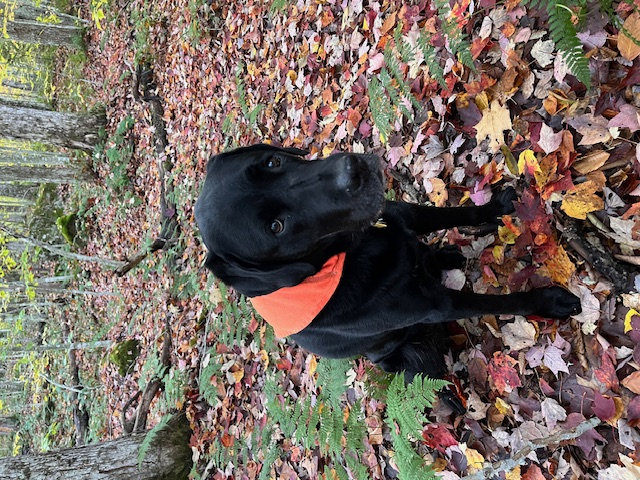
\includegraphics[width=2.08333in,height=\textheight,keepaspectratio]{documentation/images/gus.jpg}

}

\caption{Gus the lab mascot}

\end{figure}%

\bookmarksetup{startatroot}

\chapter{Process Overview}\label{process-overview}

\bookmarksetup{startatroot}

\chapter{Description of Chapter 2.}\label{description-of-chapter-2.}

\bookmarksetup{startatroot}

\chapter*{References}\label{references}
\addcontentsline{toc}{chapter}{References}

\markboth{References}{References}

Coming soon!

\phantomsection\label{refs}
\begin{CSLReferences}{0}{1}
\end{CSLReferences}




\end{document}
